\section{moeo\-GDominance\-Objective\-Vector\-Comparator$<$ Objective\-Vector $>$ Class Template Reference}
\label{classmoeoGDominanceObjectiveVectorComparator}\index{moeoGDominanceObjectiveVectorComparator@{moeoGDominanceObjectiveVectorComparator}}
This functor class allows to compare 2 objective vectors according to g-dominance.  


{\tt \#include $<$moeo\-GDominance\-Objective\-Vector\-Comparator.h$>$}

Inheritance diagram for moeo\-GDominance\-Objective\-Vector\-Comparator$<$ Objective\-Vector $>$::\begin{figure}[H]
\begin{center}
\leavevmode
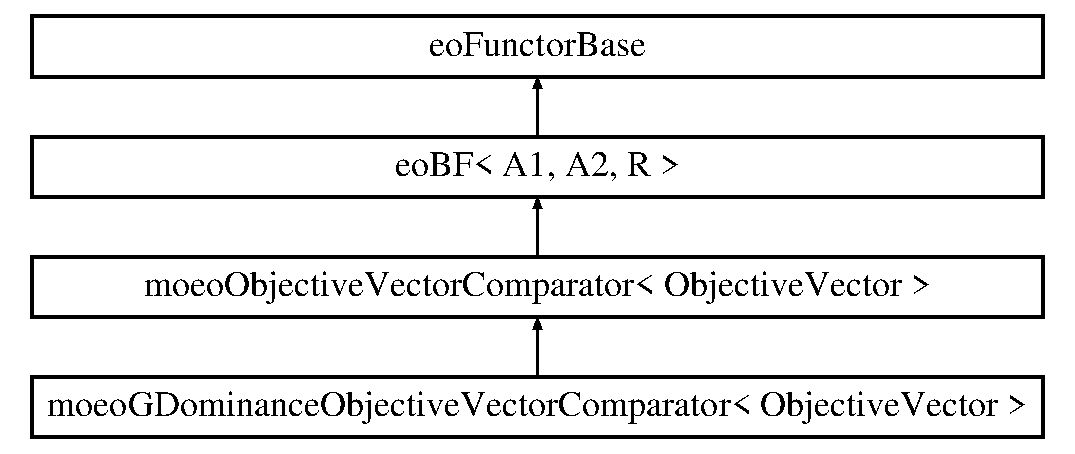
\includegraphics[height=4cm]{classmoeoGDominanceObjectiveVectorComparator}
\end{center}
\end{figure}
\subsection*{Public Member Functions}
\begin{CompactItemize}
\item 
\bf{moeo\-GDominance\-Objective\-Vector\-Comparator} (Objective\-Vector \&\_\-ref)
\begin{CompactList}\small\item\em Ctor. \item\end{CompactList}\item 
const bool \bf{operator()} (const Objective\-Vector \&\_\-objective\-Vector1, const Objective\-Vector \&\_\-objective\-Vector2)
\begin{CompactList}\small\item\em Returns true if \_\-objective\-Vector1 is g-dominated by \_\-objective\-Vector2. \item\end{CompactList}\end{CompactItemize}
\subsection*{Private Member Functions}
\begin{CompactItemize}
\item 
unsigned int \bf{flag} (const Objective\-Vector \&\_\-objective\-Vector)
\begin{CompactList}\small\item\em Returns the flag of \_\-objective\-Vector according to the reference point. \item\end{CompactList}\end{CompactItemize}
\subsection*{Private Attributes}
\begin{CompactItemize}
\item 
Objective\-Vector \& \bf{ref}\label{classmoeoGDominanceObjectiveVectorComparator_54cf089933c4d5d70ceb931c2b97ca68}

\begin{CompactList}\small\item\em the reference point \item\end{CompactList}\item 
\bf{moeo\-Pareto\-Objective\-Vector\-Comparator}$<$ Objective\-Vector $>$ \bf{pareto\-Comparator}\label{classmoeoGDominanceObjectiveVectorComparator_5768e6444e546f1da2f36ccabcfc1f70}

\begin{CompactList}\small\item\em Pareto comparator. \item\end{CompactList}\end{CompactItemize}


\subsection{Detailed Description}
\subsubsection*{template$<$class Objective\-Vector$>$ class moeo\-GDominance\-Objective\-Vector\-Comparator$<$ Objective\-Vector $>$}

This functor class allows to compare 2 objective vectors according to g-dominance. 

The concept of g-dominance as been introduced in: J. Molina, L. V. Santana, A. G. Hernandez-Diaz, C. A. Coello Coello, R. Caballero, \char`\"{}g-dominance: Reference point based dominance\char`\"{} (2007) 



Definition at line 25 of file moeo\-GDominance\-Objective\-Vector\-Comparator.h.

\subsection{Constructor \& Destructor Documentation}
\index{moeoGDominanceObjectiveVectorComparator@{moeo\-GDominance\-Objective\-Vector\-Comparator}!moeoGDominanceObjectiveVectorComparator@{moeoGDominanceObjectiveVectorComparator}}
\index{moeoGDominanceObjectiveVectorComparator@{moeoGDominanceObjectiveVectorComparator}!moeoGDominanceObjectiveVectorComparator@{moeo\-GDominance\-Objective\-Vector\-Comparator}}
\subsubsection{\setlength{\rightskip}{0pt plus 5cm}template$<$class Objective\-Vector$>$ \bf{moeo\-GDominance\-Objective\-Vector\-Comparator}$<$ Objective\-Vector $>$::\bf{moeo\-GDominance\-Objective\-Vector\-Comparator} (Objective\-Vector \& {\em \_\-ref})\hspace{0.3cm}{\tt  [inline]}}\label{classmoeoGDominanceObjectiveVectorComparator_fc4e1f1201b6420d206b28ab98e9ea0d}


Ctor. 

\begin{Desc}
\item[Parameters:]
\begin{description}
\item[{\em \_\-ref}]the reference point \end{description}
\end{Desc}


Definition at line 33 of file moeo\-GDominance\-Objective\-Vector\-Comparator.h.

\subsection{Member Function Documentation}
\index{moeoGDominanceObjectiveVectorComparator@{moeo\-GDominance\-Objective\-Vector\-Comparator}!operator()@{operator()}}
\index{operator()@{operator()}!moeoGDominanceObjectiveVectorComparator@{moeo\-GDominance\-Objective\-Vector\-Comparator}}
\subsubsection{\setlength{\rightskip}{0pt plus 5cm}template$<$class Objective\-Vector$>$ const bool \bf{moeo\-GDominance\-Objective\-Vector\-Comparator}$<$ Objective\-Vector $>$::operator() (const Objective\-Vector \& {\em \_\-objective\-Vector1}, const Objective\-Vector \& {\em \_\-objective\-Vector2})\hspace{0.3cm}{\tt  [inline]}}\label{classmoeoGDominanceObjectiveVectorComparator_4b8c3496d77abf6e774333f3296e6d79}


Returns true if \_\-objective\-Vector1 is g-dominated by \_\-objective\-Vector2. 

\begin{Desc}
\item[Parameters:]
\begin{description}
\item[{\em \_\-objective\-Vector1}]the first objective vector \item[{\em \_\-objective\-Vector2}]the second objective vector \end{description}
\end{Desc}


Definition at line 42 of file moeo\-GDominance\-Objective\-Vector\-Comparator.h.

References moeo\-GDominance\-Objective\-Vector\-Comparator$<$ Objective\-Vector $>$::flag(), and moeo\-GDominance\-Objective\-Vector\-Comparator$<$ Objective\-Vector $>$::pareto\-Comparator.\index{moeoGDominanceObjectiveVectorComparator@{moeo\-GDominance\-Objective\-Vector\-Comparator}!flag@{flag}}
\index{flag@{flag}!moeoGDominanceObjectiveVectorComparator@{moeo\-GDominance\-Objective\-Vector\-Comparator}}
\subsubsection{\setlength{\rightskip}{0pt plus 5cm}template$<$class Objective\-Vector$>$ unsigned int \bf{moeo\-GDominance\-Objective\-Vector\-Comparator}$<$ Objective\-Vector $>$::flag (const Objective\-Vector \& {\em \_\-objective\-Vector})\hspace{0.3cm}{\tt  [inline, private]}}\label{classmoeoGDominanceObjectiveVectorComparator_75bf5141369522563e60d4e3ac2ec9cb}


Returns the flag of \_\-objective\-Vector according to the reference point. 

\begin{Desc}
\item[Parameters:]
\begin{description}
\item[{\em \_\-objective\-Vector}]the first objective vector \end{description}
\end{Desc}


Definition at line 76 of file moeo\-GDominance\-Objective\-Vector\-Comparator.h.

References moeo\-GDominance\-Objective\-Vector\-Comparator$<$ Objective\-Vector $>$::ref.

Referenced by moeo\-GDominance\-Objective\-Vector\-Comparator$<$ Objective\-Vector $>$::operator()().

The documentation for this class was generated from the following file:\begin{CompactItemize}
\item 
moeo\-GDominance\-Objective\-Vector\-Comparator.h\end{CompactItemize}
